\newpage
\section{零售管理系统}
\label{sec:foundation}

\subsection{服务器}

\begin{figure}[htbp]
	\centering
	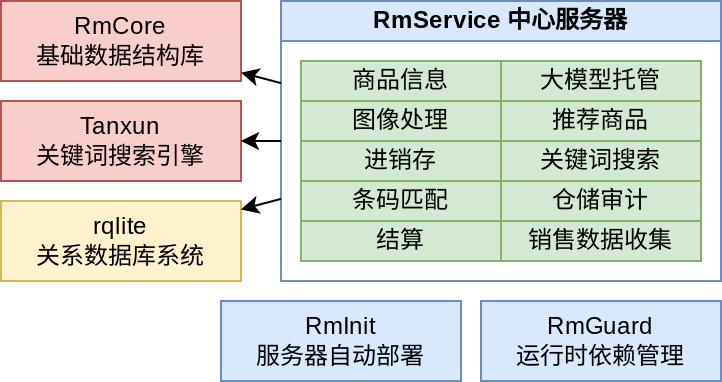
\includegraphics[width=0.8\textwidth]{./imgs/arch-server.png}
	\caption{本设计的服务器整体设计图示。其中蓝色表示相互独立的应用程序,绿色表示服务器的功能,红色表示功能库,黄色表示第三方库或应用程序,箭头表示被指方受到依赖。}
	\label{fig:arch-server}
\end{figure}

\subsubsection{数据结构}
如图 \ref{fig:arch-server} 所示,因为采用了客户端-服务器设计模式,该系统所有业务相关信息统一由RmService模块进行管理。因此,为了在系统中体现充分的可维护性、可拓展性,实际对数据进行存储的关系数据库系统rqlite原则上无法被客户端(各个商家端、顾客端应用程序)所直接访问,而是由RmCore所定义的数据结构进行封装。

\begin{figure}[htbp]
	\centering
	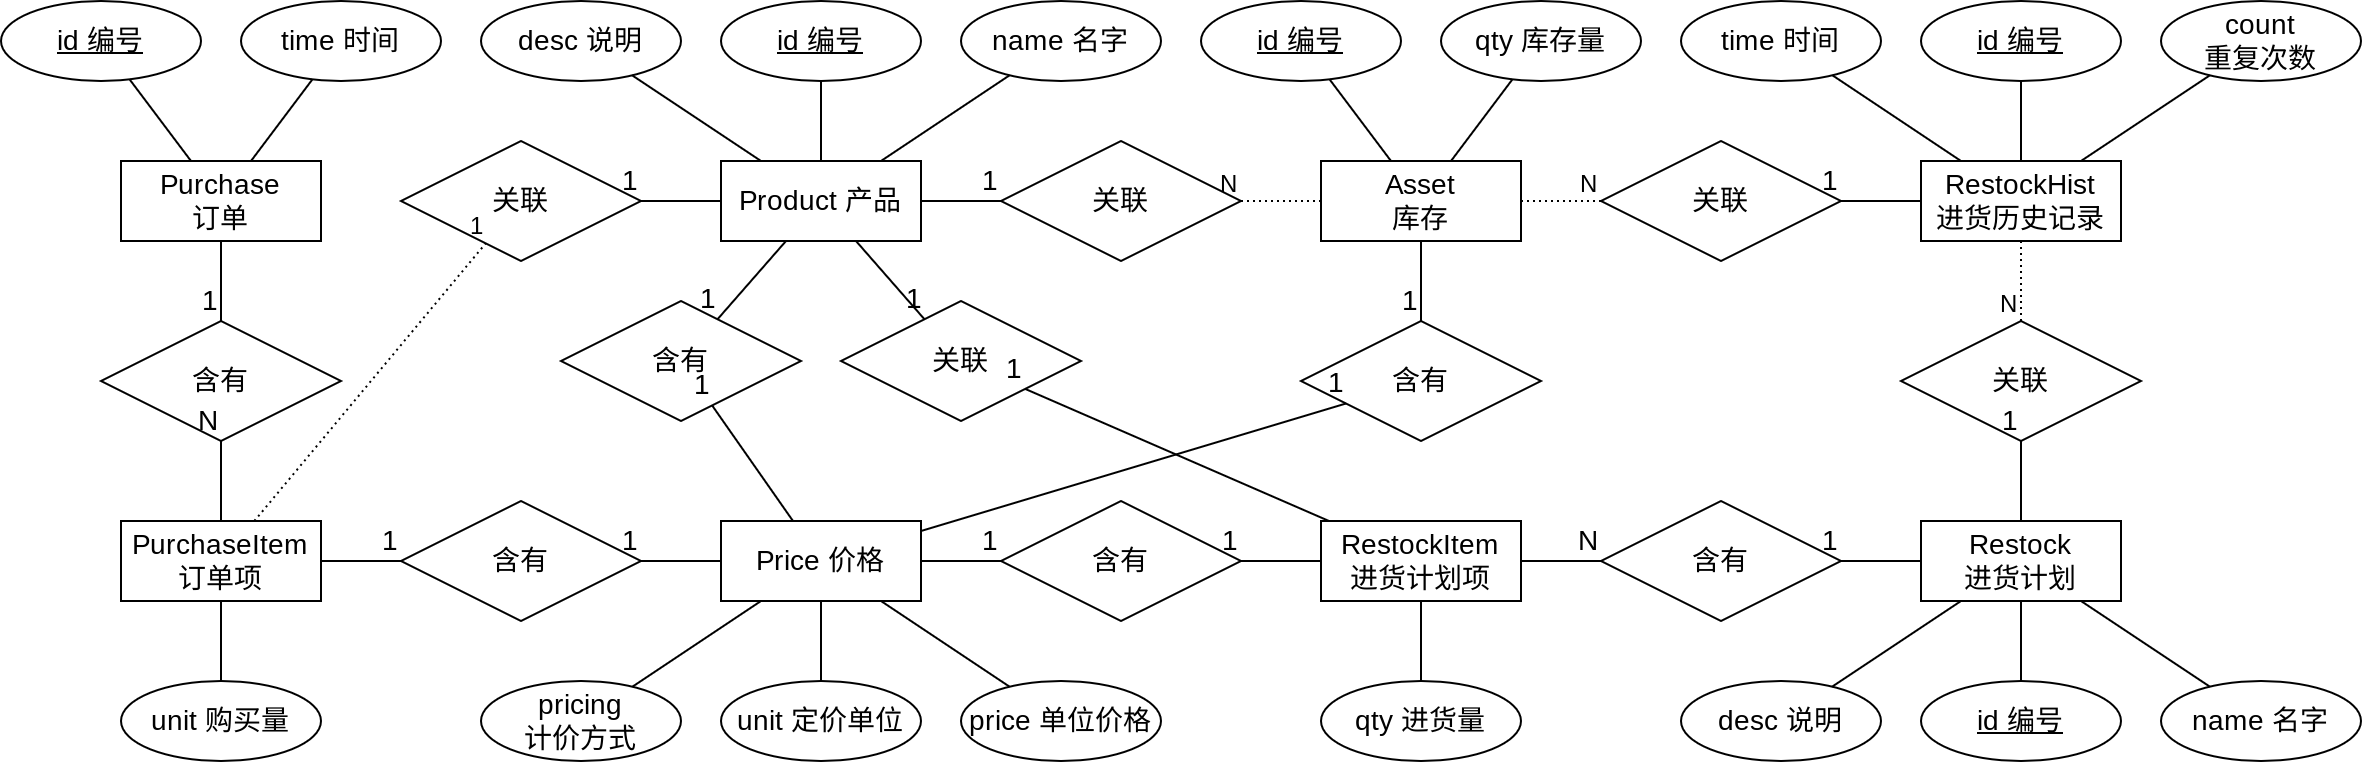
\includegraphics[width=0.8\textwidth]{./imgs/rms-er-rmcore.png}
	\caption{RmCore模块所定义数据结构的实体关系图。}
	\label{fig:rms-er-rmcore}
\end{figure}

如图 \ref{fig:rms-er-rmcore} 所示,该模块定义了在零售经营过程中会利用到的各种(需要持久化存储的)数据结构,并且已经以面向对象的、有利于代码复用、序列化和反序列化和有利于在不同开发环境下形成统一接口的方式进行封装。为了便于在数据库中以整数方式存储许多常常为小数的数据,规定任何直接代表金钱数量的值以人民币分为单位,任何直接代表物体质量的值以克为单位。

其中值得注意的一个类型是库存“Asset”。为了便于对库存所对应的进货批次、进货价格等信息进行跟踪,每一个库存项都与一个进货历史记录项目“RestockHist”相关联。因此,同一个产品可以因为多次不同进货并且较老进货批次剩余产品尚未被消化完毕而存在多个库存条目。同样地,只需要统计一个RestockHist所对应的Asset,便可以统计某一个批次进货的消化情况。

另一个较为特殊的类型是价格“Price”。考虑到不同零售商品类型定价策略的区别,该类型的属性计价方式“pricing”为具有“Package”(按件)和“Weight”(按重量)两个可能值的枚举。而属性定价单位“unit”在按件计价时代表属性价格“price”对应的商品件数,反之则是克数。而将属性price和unit分离(而不是表示为单位价格)有助于避免如“十元三件”(一件$\frac{10}{3}$元)此类出现整数或IEEE 754浮点类型数字无法准确表示的数值的情况。

\subsubsection{应用程序接口}

\subsubsection{自动部署}

\subsubsection{服务依赖管理}

\subsubsection{图像存储}

\subsection{管理界面}

\subsubsection{商品管理}

\subsubsection{库存管理}

\subsubsection{营业数据统计}

\subsubsection{其他管理功能}

\subsubsection{移动端程序}

\subsection{结算界面}

\subsubsection{条码扫描硬件}

\subsubsection{称重硬件}